\section{Experimental Setup}\label{sec:experimental-setup}

\subsection{System Configurations}\label{sec:system-configurations}
Overall the system has a three tier configuration, as it was described in the requirements. The tiers are the database machine, two middleware machines and two client machines. All the machines are t2.medium Amazon EC2 instances. In order to build the Middleware and Client applications Ant was used.
\subsection{Configuration and Deployment mechanisms}\label{sec:configuration-and-deployment-mechanisms}
For configuration of each client as mention in 2.1 the Middleware and the Client were built using Ant. In order to deploy the system including the Database and applications in each tier Python scripts were used. A main script with different function was written in order to perform different operations within the system.\\

 Moreover, fabric a python library that works as command line tool and ssh application was used as part of the deployment process see Figure \ref{fig:deploy}. In addition as part of the experiments performed in the system, when the operation that the client is not mentioned is implied that it was sending new messages to queues. This was decided as part of the performance analysis in the system in order to observer the effects of heavy task.
\subsection{Logging and Benchmarking mechanisms}\label{sec:logging-and-benchmarking-mechanisms}
\begin{figure}[h!]
	\centering
	%\def \svgscale {\columnwidt}
	
\includegraphics[scale=0.3]{logging.png}
	\caption{Different logging entry points during the lifespan of a single request in the messaging system}
	\label{logging}
	%\input{soft-mmu-2.pdf}
\end{figure}
 For the logging mechanism the library lo4j was used. The configuration files is passed as parameter to the Clients and the Middleware application. Both components log the type of request they are preforming, with a timestamp and the number of the request.\\
 
The client just before sending the request makes a log entrance and once it get the response enters a second log. In the middleware a log entrance is made when the Middleware gets the request from the client, then when it sends a request to the database and when the request returns from it, this one is to estimate the response time of the database from the middleware perspective. Finally after sending the response to the client it enters another log entrance. See Figure \ref{logging}.\\

Finally for benchmarking a python script was written in order to parse the results of the logs provided by the middleware and the clients. In addition the middleware has embedded another logging functions to log the throughput of the middleware every second during the execution of it. With those numbers in the log files and the parsing methods, a performance analysis of the system was made.

\section{Evaluation}\label{sec:evaluation}


\subsection{System Stability}\label{sec:system-stability}


In order to perform a stability test the configuration of the system was the following, the database was already initialize it had 14750 messages stored; it had a size of 324MB. Two middleware nodes, one on each t2.medium instance, 15 clients connected to each middleware node, each group of 15 client were running in a t2.medium instance as well, which makes a total of 30 clients sending and receiving data. The period of running of the experiment was for 30 minutes and with 5 repetitions in total.\\
\begin{figure}[h!]
	\centering
	%\def \svgscale {\columnwidt}
	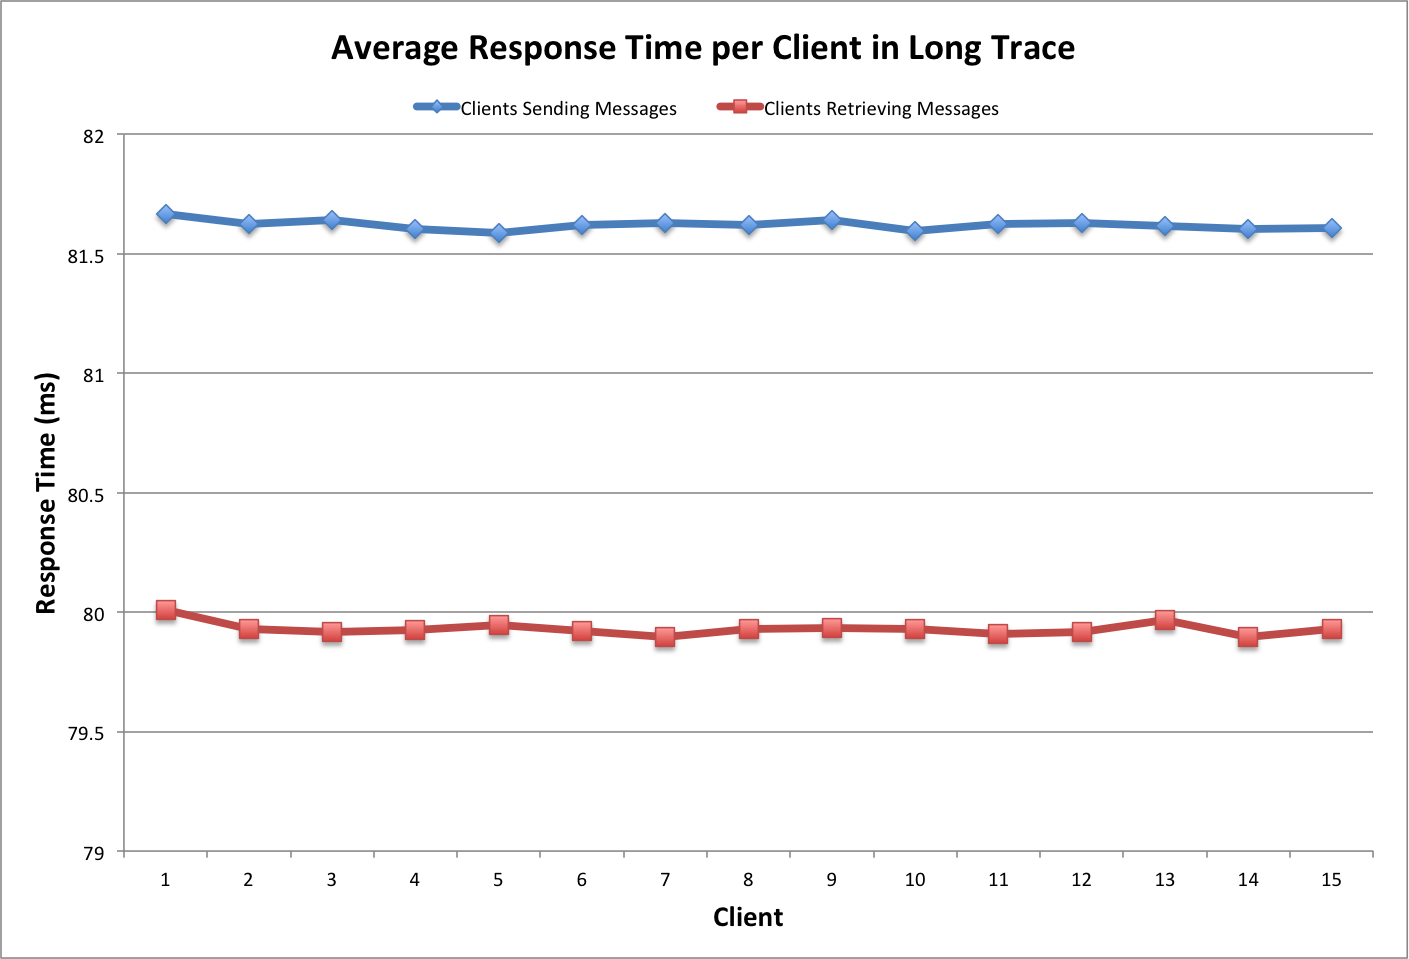
\includegraphics[scale=0.35]{stabilityRP.png}
	\caption{Plot with response time in different clients perfmorming distinct operations in the middleware}
	\label{stabilityRP}
	%\input{soft-mmu-2.pdf}
\end{figure}

From the result plotted in Figures \ref{stabilityRP} and \ref{stabilityTHR}, it can by observed in the beginning a stable throughput is observed in the system. In addition we can see the decrease of the throughput at the end in the cool down face. Furthermore there are some sparse down spikes in the throughput, which I point to the effects of the java garbage collector and the I/O activity in the middleware caused by the writing of the log files.\\
\begin{figure}[h!]
	\centering
	%\def \svgscale {\columnwidt}
	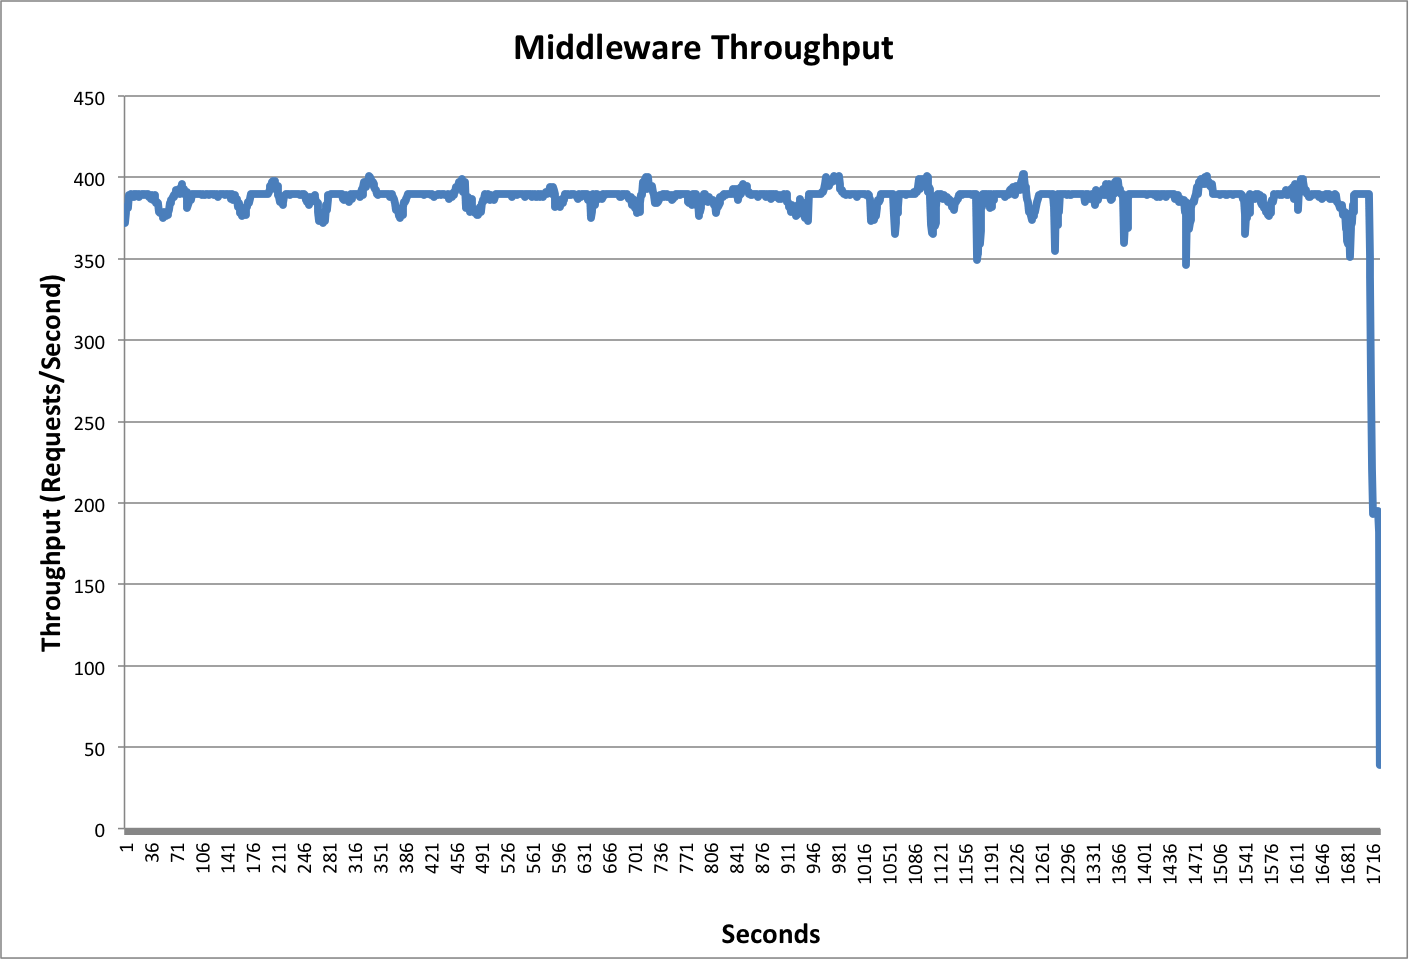
\includegraphics[scale=0.35]{stabilityTHR.png}
	\caption{Throughput during stability run over 30 minutes}
	\label{stabilityTHR}
	%\input{soft-mmu-2.pdf}
\end{figure}
In addition to the analysis of the throughput we can observe the difference in response time in the two different operations being performed by the clients. Clearly the system take more time in create a new message and save it on the system than in retrieving a single message. This makes sense since when a message is about to be created it check if the queue where is going to be stored exist or not and if it does not it creates that queue. This operation incurs in more time of processing then the retrieving a single message operation.


\subsection{System Throughput}\label{sec:system-throughput}
For the Throughput analysis five machines were used 1 database, 2 middleware and 2 client machines. Each client machine was running several client instances sending new messages to the system. With a fixed number of Client Handlers and connections to the database. Nevertheless in order to find the maximum throughput, the load in the system was increasing by the increment of running client on each client machine. The machine were t2.medium instances.

\begin{figure}[h!]
	\centering
	%\def \svgscale {\columnwidt}
	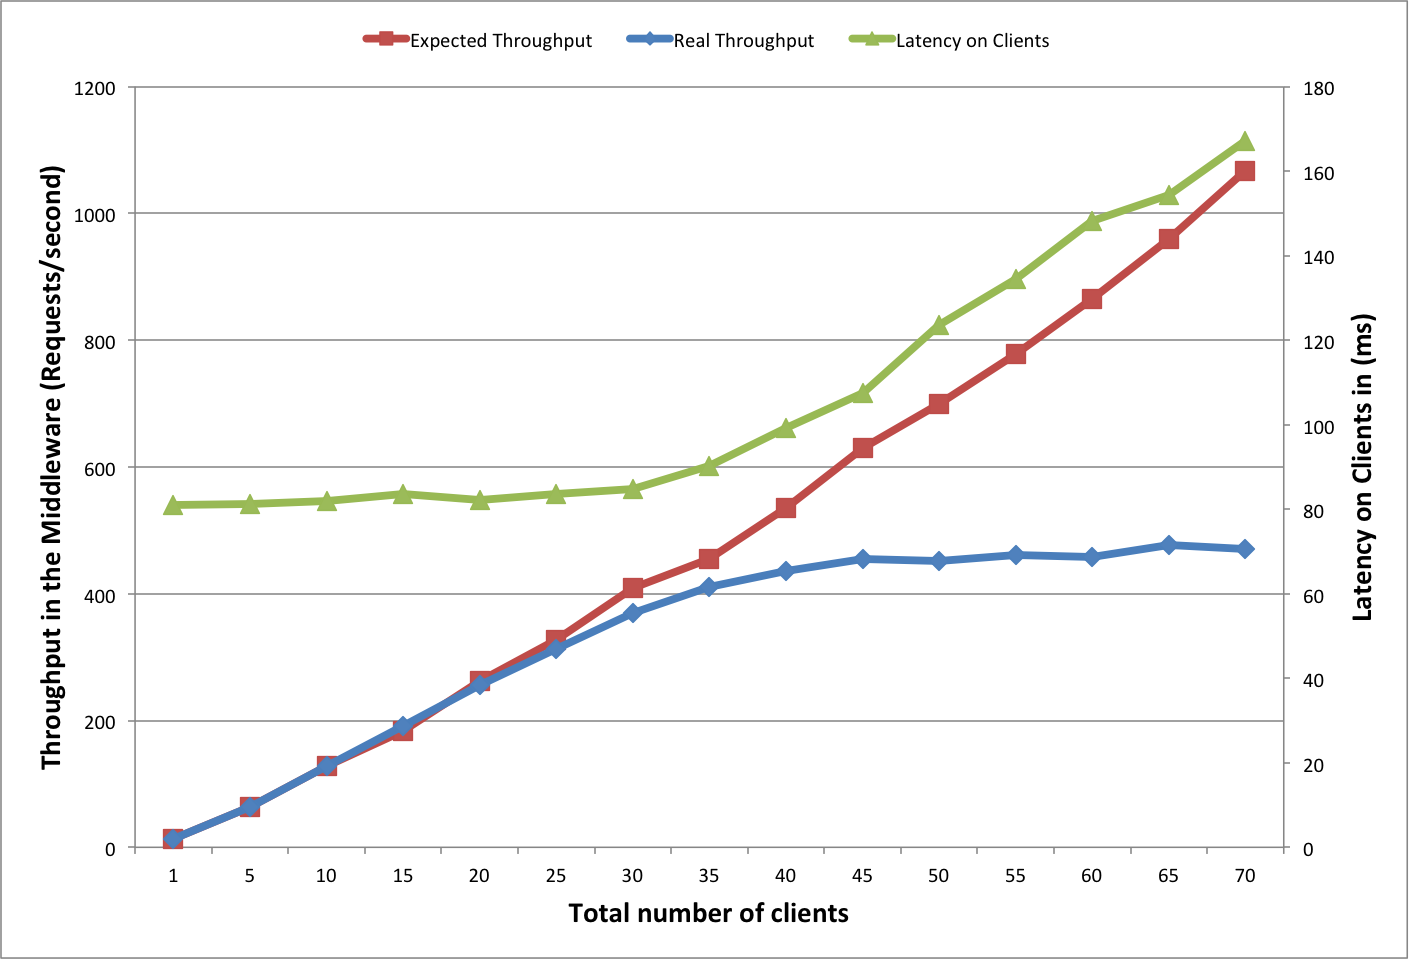
\includegraphics[scale=0.4]{through.png}
	\caption{Number of clients vs Throughput and Latency, maximum througput level achieved with incremental on response time.}
	\label{through}
	%\input{soft-mmu-2.pdf}
\end{figure}

Assuming enough resources on my system I performed experiments with increments of five clients more on each middleware on each repetition. My hypothesis for this experiment was to observe a linear increase in the throughput and to observe a constant response time.\\

Nevertheless, given the results obtained and showed in Figure \ref{through}  after preforming constant increases for periods of ten minutes I was able to find the maximum throughput on my system. In addition I was able to observe the effect that the increment of load in the system affects the response time. In the figure I plotted what I expected to be the increment in the throughput. However when the middleware is handling more than forty clients the throughput stops increasing and remain more less constant. Nevertheless the Latency or average response time that the clients are having just continues increasing.\\

Even when the Middleware is configured to handle more clients with an initial configuration running a hundred Client Hanlders to attend the requests from clients, the response time increases because of the number of connections to the database, which in this experiment is fixed to 10, are not enough to satisfy the amount of operations the clients are requesting from the middleware. Since after each database operation a connection is being taken from the pool and when all the connections are occupied the client requests must wait until one connection gets free. This as consequence increases the response time in the clients.\\

Is important to mention that the data and plot reflect only one of the middleware and the response time of a single machine running clients. Nevertheless given the fact that in both machines the clients are preforming the same operation and both middleware have the exact same configuration the same analysis and results apply for the other components.

\subsection{System Scalability}\label{sec:system-scalability}

For the scalability tests I performed a scale-up and a scale out experiments. My hypothesis for these experiments was to expect the same behavior for both and observe a constant function measured metric response time or latency, in my clients.\\

In the scale up setting the configuration of my system was a single machine running client, one middleware machine with a middleware node and my database machine. The parameters I fixed in this experiment were the number clients with 15 clients, 5 Client Handlers in the middleware and 5 connections to the database in the middleware. The experiment was running for 10 minutes, and each client was running for 3 minutes and all the clients where sending new messages of 200 character to the system.\\

For the scaling setting I was increasing by doubling value of the parameters in my system. Therefore as part of my hypothesis I was expecting to see a double increment of my throughput in the system. The result of the scale up can be observer in the Table \ref{scaleup}.\\

\begin{table*}[h]\centering
         % \ra{1.3}
         % \tabcolsep=0.5cm
         \scalebox{0.8}{
         \begin{tabular}{@{}cccc@{}}
                  \toprule
                  $Setting$ & 5 Client Handlers   & 10 Client Handlers & 20 Client Handler\\
                  
                  $/Metric$ & 15 Clients         & 30 Clients        & 60 Clients  \\
                  \cmidrule{2-4}
                 
			         Latency (ms)        & 80.22654714        & 80.25648836       & 81.48056189 \\
			         Throuhput (Req/sec) & 194.4534884        & 388.494186        & 766.6140351 \\
                  \bottomrule
                  \end{tabular}
         }
         \caption{Scalep up setting with single machine, increasing constanlty connections and client handlers}
         \label{scaleup}
 \end{table*}
 In the scaling out setting I wanted to achieve the same numbers with double incremental of my parameters. Therefore I used the same configuration for my 1 machine running clients, 1 middleware and 2 database running 15 clients, with 5 Client Handlers and 5 connections to the database and perform double value incremental having setting with 2 machines running clients, 2 middleware servers, then a final setting with 4 client machines, and 4 middleware server. Each single machine replicated was running with the same fixed values for the parameters, which were mentioned previously. The result of the scale out setting can be observer in the Table \ref{scaleout}.\\
 
\begin{table*}[h]\centering
         % \ra{1.3}
         % \tabcolsep=0.5cm
         \scalebox{0.8}{
         \begin{tabular}{@{}cccc@{}}
                  \toprule
                  $Setting$ & 1 Middleware	&2 Middlewares	&4 Middlewares\\
                  
                  $/Metric$ & 15 Clients         & 30 Clients        & 60 Clients  \\
                  \cmidrule{2-4}
					Latency (ms)&	80.22654714	&80.33796634	&81.48632835\\
					Throuhput (Req/sec)&	194.4534884	&388.3139535	&755.4543636\\
                  \bottomrule
                  \end{tabular}
         }
         \caption{Scaling out setting with fixed paramters in connections and client handlers but constant incremental of middleware nodes and client machines}
         \label{scaleout}
 \end{table*} 
 
 \begin{figure}[h]
  
 \begin{subfigure}{0.5\textwidth}
 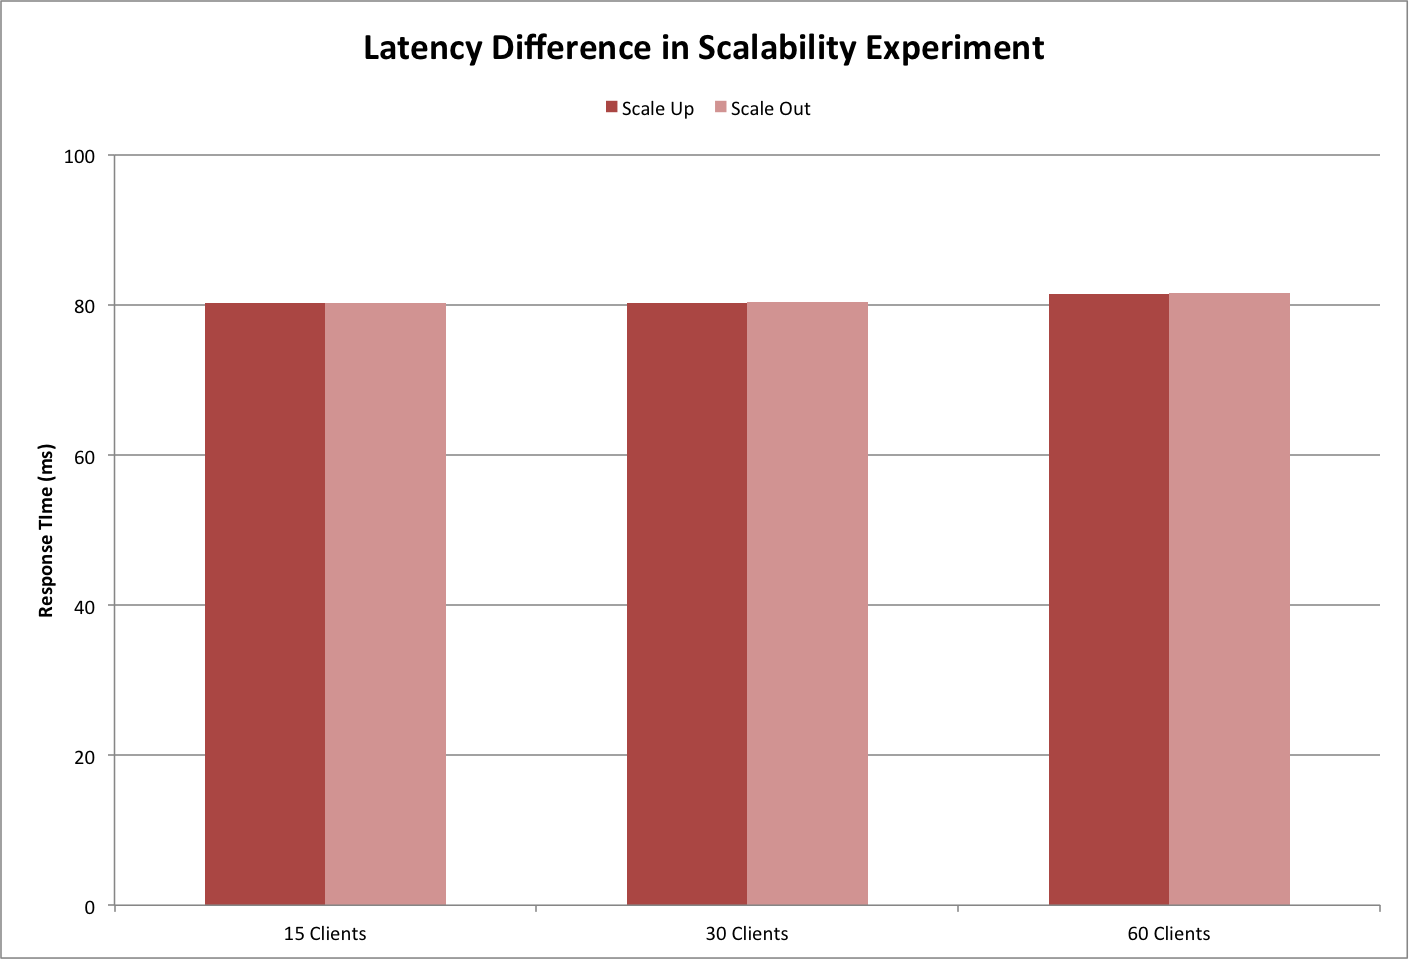
\includegraphics[width=0.9\linewidth, height=5cm]{scalRP.png} 
 \caption{Latency comparison between scaling experiments increasing number of Handlers and connections to the database in the Middleware}
 \label{fig:subim1}
 \end{subfigure}
 \begin{subfigure}{0.5\textwidth}
 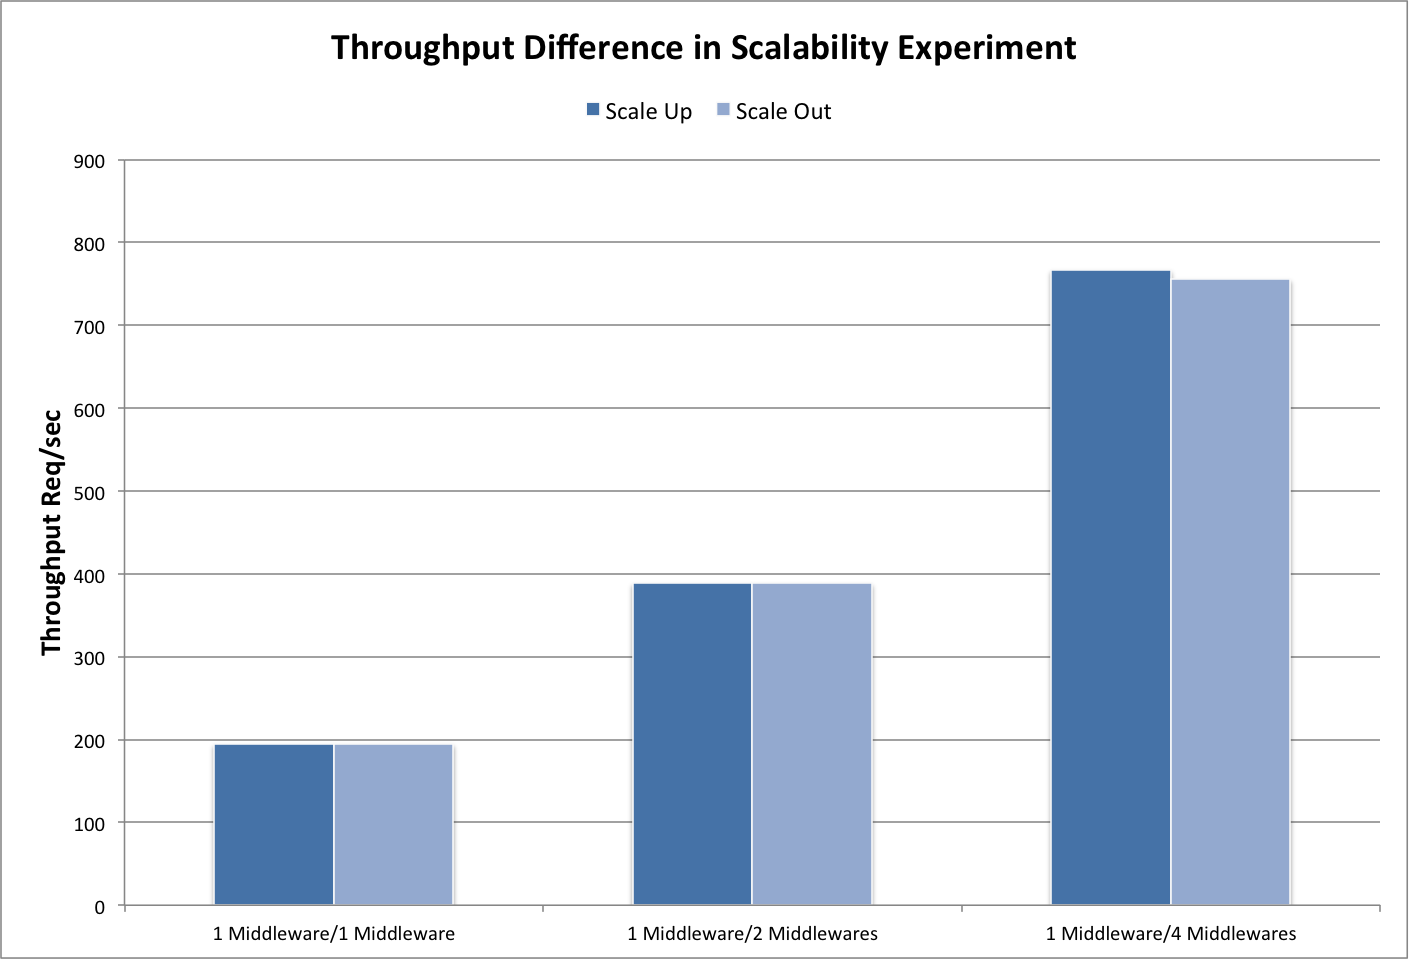
\includegraphics[width=0.9\linewidth, height=5cm]{scalTHR.png}
 \caption{Throughput comparison between scaling experiments increasing number of Handlers and connections to the database in the Middleware}
 \label{fig:subim2}
 \end{subfigure}
  
 \caption{Results in scalability experiment}
 \label{fig:image2}
 \end{figure}
As I expect on my hypothesis my system on the scaling out setting was behaving like the scale up experiment \(See Figure \ref{fig:image2}\). Nevertheless giving these scenarios, I consider scaling up factor is more efficient giving that the allocation of new requests to free connections is done by a single middleware which can be more efficient. However this may not be the case always since this depends in how the system is configured.\\

\subsection{Response Time Variations}\label{sec:response-time-variations}

In this experiment I had a setting of five machines as well, 2 middleware nodes, 2 client machines and 1 database, all t2.medium instances.\\

The fixed parameters in my experiment were the number of clients on each machine with a total of 15 on each. Each client was sending messages to the system. The number of Client Handlers were 15, one for each client and 5 connections to the database. Therefore these connections were shared among the clients. The duration of this experiment was of 5 minutes with many repetitions. In addition before every run the database started empty.\\

The parameter varying in this experiment was the length of the message been sent to the database. The reason for changing the message size of was to observe the impact of it in the response time on the clients.\\

My hypothesis for this experiment was to observer an increase in the response time metric in the system. The raise on it I expected to be as consequence of the increment in the message size.\\
 
 \begin{figure}[h!]
 	\centering
 	%\def \svgscale {\columnwidt}
 	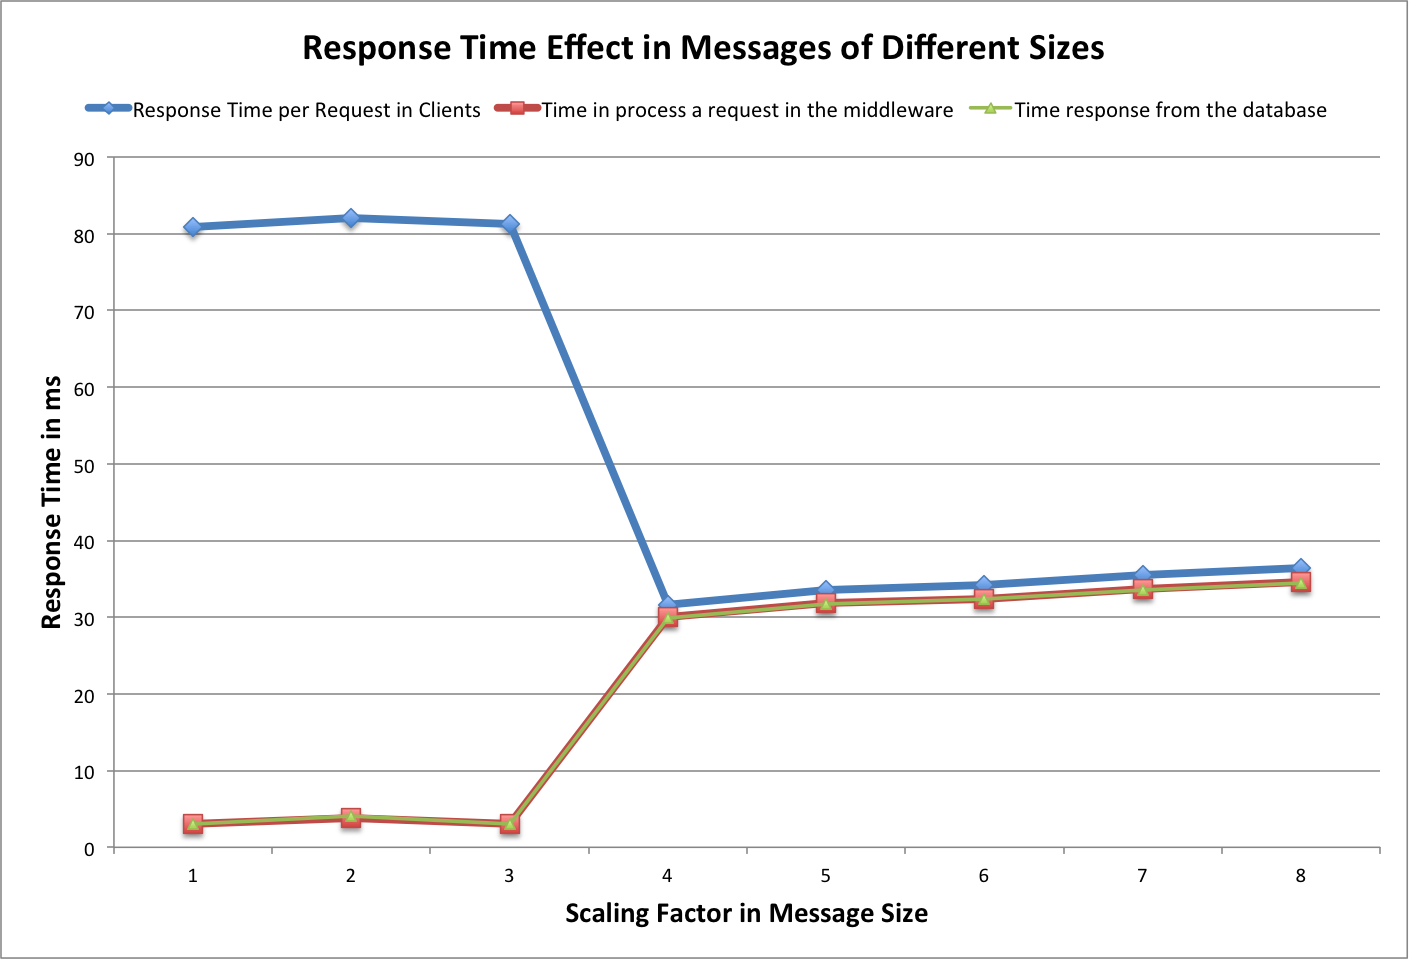
\includegraphics[scale=0.4]{response.png}
 	\caption{Response time for clients during incremental in the message size}
 	\label{response}
 	%\input{soft-mmu-2.pdf}
 \end{figure}
 
Nevertheless, after running the experiment and plot the response latency of the clients and the response time that it took for the middleware to process a request, the first results were not the ones I expected in my hypothesis. The clients were observing a high latency when the middleware time of processing a request was really low. However, after the size of the message was scaled 3 times, 600 characters, the response time in both client and middleware was behaving as expected. See Figure \ref{response}.\\

The high latency behavior of the clients observed even when the middleware is processing request fast I assume is because of what I observed is thread local allocation buffers, what is common for multi thread applications is to assign to each thread a buffer that is used only by that thread to perform allocations. When the size of the message is not big enough then the thread may assign a direct allocation to the heap requiring more synchronization. Once the size of the message is big enough then the threads optimize the use of the thread local allocation buffers (TLAB’s) with non-direct heap allocations. Improving the response time. Nevertheless in order to be 100\% certain more experiments need to be done modifying the running parameter of the Java Virtual Machine (JVM) in this case the size of the TLBA \cite{oracle}.


\subsection{$2^k$ Experiment}\label{sec:k-experiment}
For the 2\^{}k experiment the two factors I decided to explore are the number of concurrent client in my middleware (Handlers) and my number of connections in the database, the reason was because as I observed in my through put experiment by increasing the number of clients in the system in the handler parameter the throughput was increasing. Furthermore I wanted to see the impact on the number of connection has on the system.\\

Both parameters were explored in two levels each with the values of 10 and 20. As result I had to preform the experiment 4 times with adjusting the values of the previous parameters. Each experiment was running for 10 minutes, with t2.medium instances each client with and average workload of 12 requests per second.
By performing this experiment we are able to see the impact of these factors in the performance of the system in Request completed by second (Req/sec).

After the data seen in Table \ref{2k}, I define my two variables $x_{a}$ and $x_{b}$



\begin{table*}[h]\centering
         % \ra{1.3}
         % \tabcolsep=0.5cm
         \scalebox{0.8}{
         \begin{tabular}{@{}rrcc@{}}
                  \toprule
                    & \multicolumn{3}{c}{Connection to Database} \\
                  \cmidrule{2-4}
                   \multicolumn{1}{c}{$Client Hanlder$} &&$10$ &$20$\\
                  \midrule 
			         10 &&$129.354782609$&$128.763478261$   \\
			          20 &&$257.597560976$&$258.93554007$   \\
                  \bottomrule
                  \end{tabular}
         }
         \caption{Throughput metric results for different settings of the $2^k $ experiment}
         \label{2k}
 \end{table*}  
 
 $$x_{a}=\begin{cases} -1& if\quad 10 \quad Connections\quad  to\quad  Dabatase\\1 & if\quad 20 \quad Connections\quad  to\quad  Dabatase\end{cases}\\
 $$
 $$x_{b}=\begin{cases} -1& if\quad 10 \quad Client\quad Hanlders\\1 & if\quad 20 \quad Client\quad Hanlders\end{cases}$$
 After the analysis of my results my hypothesis about the number of Client Handler impacting in high way the performance of my system is true. Furthermore I was able to show that given the current configuration of my database and the number of connections it has is more than enough for my system.\\
 
Furthermore my $2^k$ experiment show that the mean request per second is $193.6628405$, in addition the impact of the connection in request per second of my database connections is very low $ 0.186668686$ requests per second. However the value in my number of Client Handlers accounts for $ 64.60371004$ Requests per second. Finally the interaction of these two combined have an effect of $ 0.482320861$ Request per Second.See Table \ref{2kr}.


\begin{table*}[h]\centering
         % \ra{1.3}
         % \tabcolsep=0.5cm
         \scalebox{0.8}{
         \begin{tabular}{@{}rrrrr@{}}
         \toprule
         
          & \multicolumn{3}{c}{Design of $2^2$ Experiment} \\
         \cmidrule{1-5}

         I           & A           & B           & AB          & y           \\
         \midrule 
         1           & -1          & -1          & 1           & 129.3547826 \\
         1           & 1           & -1          & -1          & 128.7634783 \\
         1           & -1          & 1           & -1          & 257.597561  \\
         1           & 1           & 1           & 1           & 258.9355401 \\
         774.6513619 & 0.746674746 & 258.4148402 & 1.929283442 & Total       \\
         193.6628405 & 0.186668686 & 64.60371004 & 0.482320861 & Total/4  \\
         \bottomrule  
         \end{tabular}
         }
         \caption{Wieghts on the response variables}
         \label{2kr}
         
 \end{table*}  
 $$SSM=2^2(0.186668686^2+64.60371004^2+0.482320861^2)=16695.62732$$
 $Accountability \quad of \quad components$\\
 $A=0.000834834\%$	$B=99.99359165\%$	$AB=0.005573517\%$\\
 

In addition to my fist 2\^{}k experiment I decided to run a second design for a 2\^{}k experiment. This was inspired by the results I obtained in my scalability test. I wanted to know how much the number of clients and the numbers of middleware nodes affect the performance of my system in this case the throughput. Clearly in my scalability experiment in increasing the load the throughput was increasing. However as part of the scalability experiment, the number of Client Handlers where increasing and the number of connections of the database as well.\\ 

In this experiment overall this previous parameters will remain fixed and the only changing parameter changing in a two level scale will be the number of client and the number of Middleware nodes. The experiment configuration is the following:\\

All machines are t2.medium instances, the time of the experiment is 10 minutes, with fixed values overall configuration of 20 client handlers, 10 database connections, with a message of 1600 character, all clients are running in sending mode which is sending new messages to the database into the queues.\\

The 2\^{}k parameters are the number of clients with 20, and 40 and the number of middleware nodes with 1 and 2. My hypothesis for this experiment is to observer a constant performance in throughput on both settings. In addition I expect that the parameter that account more for the throughput will be the number of clients like I in the maximum throughput experiments. This as long as there is enough Client Handlers in the system to attend the clients.\\

\begin{table*}[h]\centering
         % \ra{1.3}
         % \tabcolsep=0.5cm
         \scalebox{0.8}{
         \begin{tabular}{@{}rrcc@{}}
                  \toprule
                    & \multicolumn{3}{c}{Middleware Nodes} \\
                  \cmidrule{2-4}
                   \multicolumn{1}{c}{$Clients$} &&$1$ &$2$\\
                  \midrule 
			         20 &&$455.1$&$	814.6061498$   \\
			          40 &&$928.9178571$&$	1735.999362$   \\
                  \bottomrule
                  \end{tabular}
         }
         \caption{Throughput metric results for different settings of the $2^k $ experiment with clients and middlewares}
         \label{2k2}
 \end{table*}  
 
 $$x_{a}=\begin{cases} -1& if\quad 20 \quad Clients  \\1 & if\quad 40 \quad Clients\end{cases}\\
 $$
 $$x_{b}=\begin{cases} -1& if\quad 1 \quad Middleware\\1 & if\quad 2 \quad Middleware\end{cases}$$
 \begin{table*}[h]\centering
          % \ra{1.3}
          % \tabcolsep=0.5cm
          \scalebox{0.8}{
          \begin{tabular}{@{}rrrrr@{}}
          \toprule
          
           & \multicolumn{3}{c}{Design of $2^2$ Experiment} \\
          \cmidrule{1-5}
 
          I           & A           & B           & AB          & y           \\
          \midrule 
          1           & -1          & -1          & 1           & 455.1 \\
          1           & 1           & -1          & -1          & 814.6061498 \\
          1           & -1          & 1           & -1          & 928.9178571  \\
          1           & 1           & 1           & 1           & 1735.999362 \\
          3934.623368 &	1166.587654	& 1395.211069 &	447.5753546 & Total       \\
          983.6558421 &	291.6469135	& 348.8027672 &	111.8938386 & Total/4  \\
          \bottomrule  
          \end{tabular}
          }
          \caption{Wieghts on the response variables}
          \label{2kr2}
          
  \end{table*}  
  
  $$SSM=2^2(85057.92218^2+121663.3704^2+12520.23113^2)=876966.0949$$
   $Accountability \quad of \quad components$\\
   $A=38.79644729\%$	$B=55.49285024\%$	$AB=5.710702477\%$\\
   
   After performing the experiment I find out that my hypothesis was not true, even in the setting where both configurations had the same amount of clients, the setting with 2 middleware nodes had a higher throughput. As conclusion for this experiment this behavior was due to the constant values in the client handler and connections to the database. In the scalability experiment that throughput was the same in both single middleware and multiple one because the previous mentioned parameter where also increasing as part of the scalability test and in this one they remain constant. Finally in this setting the Middleware component has a higher impact in the throughput of the system.
\subsection{Conclusion}\label{sec:conclusion}
The messaging system has many components that clearly affects it performance. Furthermore different results could be observed given a different fixed parameters. On my system given a robust database, the middleware system was not enough to stress out the performance of it. The main component affecting the throughput of my system was the number of Connection Handlers. This was observed in the maximum throughput experiment and the 2\^{}k analysis also supported that assumption. As result my bottleneck was in the number of handlers. However not necessary increasing this number will always improve the performance. This is because the machine has fixed amount of resources and by increasing the number of handlers also increases the switching on memory assigned asnd more parameters that may affect the system.\\

The workload on my system was proportional to the number of clients been handled by the system simultaneously. However the number of clients was also limited by the memory assigned for thread in the machine. In my case with a number above of 66 clients the memory was already consumed. This could be fixed by increasing the memory assigned for thread in the machine. In the system my arrival rate and my completion rate were equal since this is a closed system and I couldn’t have a new request before completing the previous one.\\

Finally, If could design my system anew the component I will change the normal network communication instead of using the normal sockets and the Object Data streamers I would use the non-blocking and buffered oriented sockets to improve the performance and avoid for example the behavior observed in the response time experiment with small size messages. In addition I would use bigger and more powerful machines in order to generate enough load such that the database performance could be affected in a more significant way.\\

